\documentclass[12pt]{article}
\usepackage{mathtools}
\usepackage{tikz}
\usetikzlibrary{matrix}
\title{CS303 Data Structures Assignment \#1\\
\large attachments and source available at https://github.com/alexskc/cs303}
\author{Aleksander Charatonik}
\begin{document}

\maketitle

\section{}
{\small
Choose an arbitrary \(n_0\), eg. \(n_0=1\).

\(Cn_0^3>n_0^3-5n_0^2+20n_0-10\)

\(C*1^3>1^3-5*1^2+20*1-10\)

\(C>1-5+20-10\)

\(C=6, n_0=1\)\\
}
For all \(n\), where \(n>1\), \(6n^3>n^3-5n^2+20n-10\).\\

\section{}
See attached \texttt{comparegrowth.cpp}. Output:\\
\texttt{
y1: 10\\
y2: 2\\
y1: 1010\\
y2: 502\\
y1: 2010\\
y2: 2002\\
y1: 3010\\
y2: 4502\\
y1: 4010\\
y2: 8002\\
y1: 5010\\
y2: 12502\\
y1: 6010\\
y2: 18002\\
y1: 7010\\
y2: 24502\\
y1: 8010\\
y2: 32002\\
y1: 9010\\
y2: 40502\\
y1: 10010\\
y2: 50002\\
}

The results here are to be expected. y1 is initially larger because of the constant 100 rather than 5, but y2 quickly overtakes it because of how much faster \(n^2\) grows than \(n\). This would be true regardless of what constant y1 used. If \(y1=10000n +20\), y2 would still outgrow it.\\

\section{}
\subsection{}
The inner loop is run \(i^2\) times, with i being every number from 0 to n-1. Therefore, we get the sum:
\(T(n)=1^2+2^2+3^2\dots+n^2\) or\\
\(T(n)=\displaystyle\sum_{i=1}^n i^2\), which is simply a geometric series, so \(T(n)=\frac{1}{6}n(n+1)(2n+1)\), or \(O(n)=n^3\).
\subsection{}
This is the same as a simple "i to n" loop, but backwards, which makes no difference, and skipping every other number, which halves the iterations. For loops with odd numbers, we get to 1, and then decrement again, so we take the ceiling of that fraction.\\
\(T(n)=\lceil\frac{1}{2}n\rceil\), and \(O(n)=n\).\\
\subsection{}
This is similar to \ref{3.1}, except instead of subcracting, we're dividing. So, instead of dividing i, we use the logarithm. We have to add one, because we continue to divide after getting to 2, and we take the floor because numbers that aren't powers of two will fall just faster than the power of two above them.\\
\(T(n)=\lfloor\log 1+1\rfloor+\lfloor\log 2+1\rfloor+\lfloor\log 3+1\rfloor\dots\lfloor\log n+1\rfloor\).\\
\(T(n)=\displaystyle\sum_{i=1}^n \lfloor\log i+1\rfloor\)\\
This can be imagined as \(1+2+2+3+3+3+3+4+4+4+4+4+4+4+4+5\dots\), where the number jumps up every time \(\log i\) returns a whole number. Every power of two. So \(T(n)=\displaystyle\sum_{i=1}^n i*2^{i-1}\) and \(T(n)=n2^n-2^n+1\). \(O(n)=n2^n\).\\

\section{}
pop\_back() removes the last element in the vector. So we'd remove the element \texttt{5} at location \texttt{4} in that vector, resulting in an array like this:

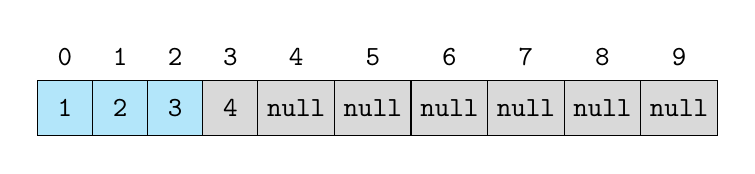
\begin{tikzpicture}
  [font=\ttfamily,
array/.style={matrix of nodes,nodes={draw, minimum size=7mm, fill=gray!30},column sep=-\pgflinewidth, row sep=0.5mm, nodes in empty cells,
  row 2 column 1/.style={nodes={fill=cyan!30}},
  row 2 column 2/.style={nodes={fill=cyan!30}},
  row 2 column 3/.style={nodes={fill=cyan!30}},
  row 1/.style={nodes={draw=none, fill=none, minimum size=5mm}}}]
  \matrix[array] (array) {
    0 & 1 & 2 & 3 & 4 & 5 & 6 & 7 & 8 & 9\\
    1 & 2 & 3 & 4 & null & null & null & null & null & null \\};
\end{tikzpicture}\\
with the\_data pointing to that array for both v1 and v2.
\end{document}
